\section{Introduction}

World-action models (WAMs) integrate future-observation prediction with robot control. Recent systems such as DreamZero~\cite{ye2026world}, DVA~\cite{rhoda2026dva} and LingBot-VA~\cite{li2026causal, lingbotva2} use pretrained video models to couple future-observation prediction with robot action generation. However, differences in their backbones, training data, objectives, and inference procedures make it difficult to isolate the effect of video--action interaction.

\begin{figure*}[t]
  \centering
  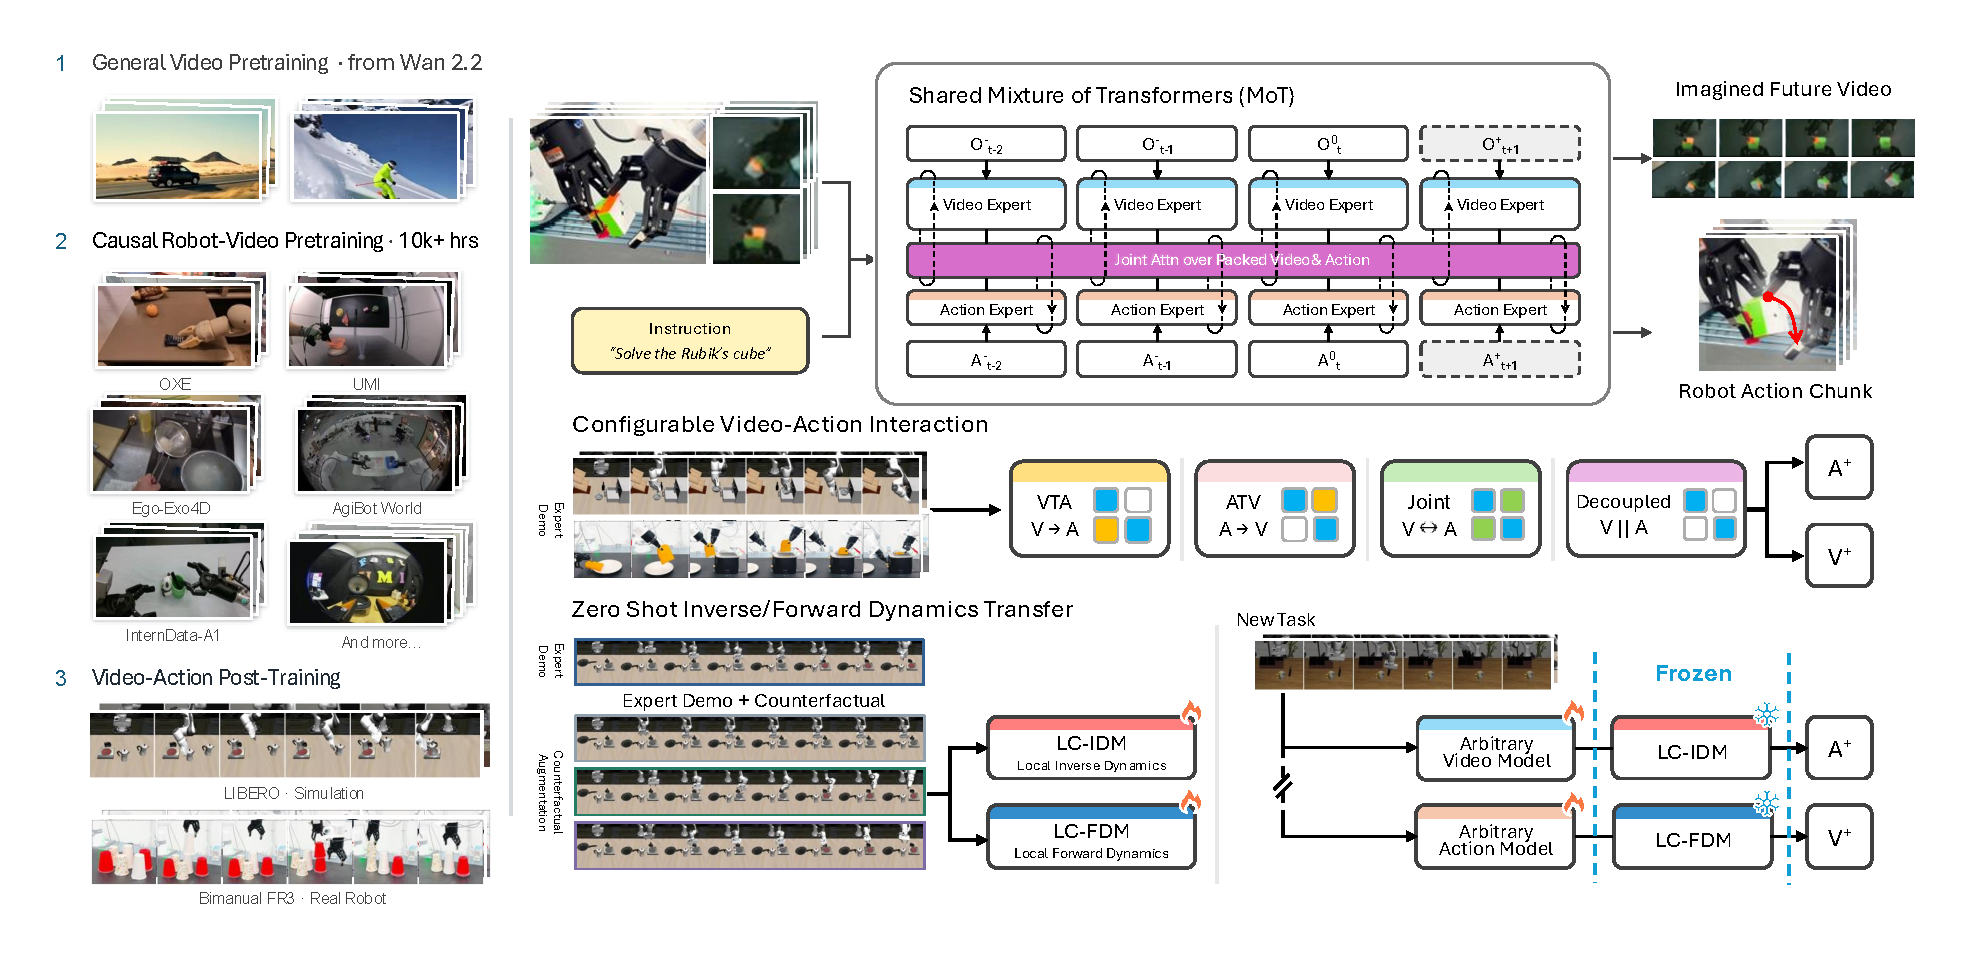
\includegraphics[width=0.98\textwidth]{sec/images/openwam-fig1-combined-v4.pdf}
  % \vspace{-0.3in}
  \caption{
\textbf{Overview of \ours.}
\textbf{Left:} Starting from Wan2.2~\cite{wan2025wan}, causal pretraining on robot and
human-interaction video builds a predictive backbone without action labels,
followed by video--action training on simulated and real-robot demonstrations.
\textbf{Top right:} A shared Mixture-of-Transformers couples temporally
aligned video and action streams through joint attention while retaining
modality-specific experts.
\textbf{Middle right:} Configurable cross-modal attention and generation
order support joint, video-then-action, action-then-video, and decoupled
prediction within the same architecture.
\textbf{Bottom right:} Local-context inverse and forward dynamics models
are trained independently using demonstrations and counterfactual
transitions. A frozen IDM translates predictions from compatible
task-adapted video models into actions, while an FDM predicts the visual
consequences of candidate actions.
}
  \label{fig:openwam-teaser}
\end{figure*}

Two challenges arise when studying these systems systematically. First, video--action interaction spans multiple choices: video and actions can be generated jointly, sequentially, or through restricted cross-modal connections. A shared architecture and evaluation protocol would allow these interaction patterns and generation orders to be compared under controlled conditions.
Second, successful demonstrations cover only a limited subset of possible action--outcome relationships. Other interactions, including failures, exploratory behavior, and counterfactual rollouts, can provide additional supervision about local dynamics. However, it remains unclear whether such data can improve the reuse of an action-grounding component when the visual predictor is adapted to a new task. We study this question by independently training local-context dynamics models and evaluating their transfer across adapted video predictors.

To this end, we introduce \textbf{\ours}, an open framework and model series for controlled world--action modeling, summarized in Figure~\ref{fig:openwam-teaser}. Starting from a pretrained general-purpose video model, we adapt its visual prior through causal robot-video training without action labels, then introduce an action branch through a Mixture-of-Transformers (MoT) architecture~\cite{liang2024mixture}. The resulting model supports joint, sequential, and restricted video--action interaction. These configurations share the video initialization, representations, and evaluation pipeline, allowing us to compare how their interaction patterns affect the control performance.

Furthermore, \ours trains \textbf{local-context inverse and forward models} independently. The inverse model predicts actions from the current observation and a future visual trajectory, while the forward model predicts that trajectory from supplied actions.
In simulation, we broaden their training data by executing alternative action sequences from the same initial state.
% On physical robots, we supplement inverse-model training with failed attempts and free-form play.
This local-transition formulation is also compatible with failed and exploratory interactions, because it does not require a successful task outcome or a success label.
Each recorded transition supplies dynamics supervision regardless of whether it completes the task. At inference, a video predictor can propose a visual trajectory and a separately trained inverse model can translate it into executable actions.

We evaluate robot-video pretraining, closed-loop policy success across
video--action interaction modes and dynamics-component reuse. In transfer experiments, task-adapted video predictors are paired with frozen inverse models to compare demonstration-only with counterfactual-augmented supervision and local-context with full-context conditioning. We additionally evaluate forward prediction under alternative actions from the same initial state.

This work makes three contributions:
\begin{itemize}
  \item \textbf{A controlled WAM framework.} \ours combines a causal video backbone with configurable video--action models under shared training and evaluation protocols.
  \item \textbf{Local-context dynamics interfaces.} We independently train inverse- and forward-dynamics models from demonstrations and broader local transitions and evaluate their composition with separately trained predictors.
  \item \textbf{Controlled empirical analysis.} We measure the effects of robot-video pretraining, interaction design, transition coverage, and conditioning context on policy performance and component reuse.
\end{itemize}

% BEGIN ARCHIVED INTRODUCTION -- superseded 2026-09-10
% Previous approved version preserved verbatim below, with each line commented out.
% \section{Introduction}
%
% World-action models (WAMs) couple robot action generation with predictions of
% future observations, bringing video modeling into the control process. Recent
% systems such as DreamZero~\cite{ye2026world} and
% LingBot-VA~\cite{li2026causal} demonstrate how pretrained video models can
% support robot manipulation through joint or sequential video--action
% generation. These approaches motivate a common foundation for studying how
% predictive models and action generation should interact.
%
% \begin{figure*}[t]
%   \centering
%   \includegraphics[width=0.98\textwidth]{sec/images/openwam-framework-hero-v12-preview.pdf}
%   \caption{Overview of Open-WAM. Left: a three-stage curriculum transfers a general video prior through robot-video training to video-action learning. Center: a shared Mixture-of-Transformers exposes configurable video--action interaction programs and learns from both expert demonstrations and counterfactual transitions through policy/joint-denoising and strict inverse- and forward-dynamics objectives. Right: the evaluation view combines LIBERO success across four task suites with representative closed-loop rollouts. \textit{Performance values are temporary placeholders and will be replaced with final results.}}
%   \label{fig:openwam-teaser}
% \end{figure*}
%
% Two challenges arise when developing such a foundation. First, video--action
% interaction spans multiple choices: video and actions can be generated jointly,
% sequentially, or through restricted cross-modal connections. Existing systems
% combine these choices with different backbones, representations, training data,
% and inference procedures, making their effects difficult to isolate. A shared
% architecture and evaluation protocol would allow interaction patterns and
% generation order to be studied as controlled variables.
%
% Second, learning reusable dynamics requires coverage beyond the actions taken
% in successful demonstrations. Failed attempts, exploratory behavior, and
% counterfactual rollouts also contain valid action--outcome relationships. Recent
% work already exploits such experience for world modeling and policy
% improvement, including PlayWorld~\cite{yin2026playworld}, FACT~\cite{peng2026fact},
% and Motus2~\cite{bi2026motus2}. Video planning with independently trained
% inverse dynamics also has an established precedent in UniPi~\cite{du2023learning}.
% Building on these directions, we investigate how transition coverage and
% conditioning boundaries affect the reuse of dynamics components when an
% upstream video predictor is adapted to new tasks.
%
% We introduce \textbf{\ours}, an open framework and model series for controlled
% world--action modeling. Starting from a pretrained general-purpose video model,
% we adapt its visual prior through causal robot-video training without action
% labels, then introduce an action branch for video--action learning. A shared
% Mixture-of-Transformers architecture supports joint, video-then-action,
% action-then-video, and restricted-interaction configurations. Common
% representations and training, rollout, and evaluation interfaces make these
% configurations directly comparable while supporting separately trained
% components.
%
% Within this framework, we define \textbf{strict inverse and forward dynamics
% interfaces} over local transitions. The inverse dynamics model (IDM) predicts
% actions from an observed visual transition, while the forward dynamics model
% (FDM) predicts future observations from supplied actions. Both use current
% observations and proprioception without requiring task language or preceding
% history. We train these components independently using demonstrations and
% counterfactual transitions collected by executing alternative action sequences
% from the same simulator state. Each transition supplies valid dynamics
% supervision regardless of task success. At inference, a video predictor can
% provide a future trajectory to a separately trained IDM for action generation,
% allowing visual prediction and action grounding to be adapted and evaluated
% independently.
%
% We evaluate \ours through native policy performance, local dynamics
% prediction, and component reuse. Our transfer study adapts the video predictor
% while retaining source-trained IDMs, and suggests that counterfactual
% supervision improves action-component reuse across the evaluated object and
% scene changes. Complementary forward-dynamics experiments examine whether
% predictions distinguish the outcomes of alternative actions from the same
% state.
%
% Our contributions are:
% \begin{itemize}
%   \item \textbf{An open WAM framework and robot-video foundation} that support controlled comparisons of video--action interaction under a common architecture and evaluation stack.
%   \item \textbf{Strict local dynamics interfaces trained from demonstrations and counterfactual transitions}, supporting inverse and forward prediction and composition with independently trained generators.
%   \item \textbf{A systematic study of interaction design, dynamics learning, and component reuse}, including transfer with an adapted video predictor and a frozen IDM.
% \end{itemize}
%
% END ARCHIVED INTRODUCTION

% BEGIN ARCHIVED INTRODUCTION -- superseded 2026-09-09
% Previous version preserved verbatim below, with each line commented out.
% \section{Introduction}
%
% Vision-language-action (VLA) models have scaled instruction-conditioned robot
% control by transferring semantic knowledge from vision-language pretraining to
% action generation \cite{brohan2022rt, brohan2023rt, kim2024openvla, team2024octo, black2024pi_0, intelligence2025pi_}. However, their
% training objectives need not explicitly represent how an action changes the
% physical world. World-action models (WAMs) offer a complementary route: they
% couple action generation with predicted video or latent future states, using
% dense temporal supervision to make scene evolution explicit
% \cite{wu2024unleashing, cheang2024gr, ye2026world, li2026causal}. This is appealing for manipulation,
% where contact, occlusion, and delayed effects can make the consequence of an
% action as important as its semantic intent.
%
% \begin{figure*}[t]
%   \centering
%   \includegraphics[width=0.98\textwidth]{sec/images/openwam-framework-hero-v12-preview.pdf}
%   \caption{Overview of Open-WAM. Left: a three-stage curriculum transfers a general video prior through robot-video training to video-action learning. Center: a shared Mixture-of-Transformers exposes configurable video--action interaction programs and learns from both expert demonstrations and counterfactual transitions through policy/joint-denoising and strict inverse- and forward-dynamics objectives. Right: the evaluation view combines LIBERO success across four task suites with representative closed-loop rollouts. \textit{Performance values are temporary placeholders and will be replaced with final results.}}
%   \label{fig:openwam-teaser}
% \end{figure*}
%
% A WAM, however, is not a single architecture. Actions may consume explicit
% future frames, decoded visual features, intermediate video latents, auxiliary
% registers, or a parallel stream; video and action may be generated sequentially
% or jointly; and the video branch may be required at inference or used only as
% training-time supervision. Recent systems occupy different points in this
% space: DreamZero jointly denoises future video and actions, LingBot-VA follows a
% causal video-first design, Fast-WAM retains world-model supervision while
% reducing test-time imagination, and OA-WAM organizes predicted states around
% addressable objects
% \cite{ye2026world, li2026causal, yuan2026fast, liu2026oa}.
% Yet these choices are usually evaluated with different backbones, data,
% causality assumptions, action conventions, and runtime systems. Consequently,
% a higher success rate cannot be attributed cleanly to the proposed
% video--action coupling, and seemingly common benchmark results need not
% constitute matched comparisons.
%
% Comparability is only one limitation. Most robot WAMs learn primarily from
% successful, language-conditioned demonstrations. These trajectories specify
% how to complete a task, but cover only a narrow part of the possible
% observation--action--outcome distribution. Failed attempts, exploratory or
% scripted behavior, and counterfactual rollouts may not achieve an instructed
% goal, yet they still reveal how the world changes under an action. In
% particular, paired counterfactual trajectories expose alternative outcomes from
% the same initial state and provide direct supervision for local inverse and
% forward dynamics. Such interactions can be collected without requiring task
% success and need not carry language labels, but standard task-conditioned WAM
% objectives are not designed to use them directly. Action-conditioned world
% models demonstrate the value of transition-level supervision
% \cite{huang2026learning, li2025worldeval, guo2026ctrl}; the open problem is how to
% transfer that supervision into a task policy without training a separate model
% for every data source or inference role.
%
% We introduce \textbf{Open-WAM}, an open-source framework and model series for
% controlled WAM research. Its central abstraction is a \emph{video-stage
% contract}: a \emph{VisualTower} exposes observed tokens, predicted future
% latents, optional decoded futures, and runtime caches; a \emph{PolicyVariant}
% declares which stages it consumes; and an \emph{ActionDecoder} maps the selected
% representation to executable action chunks. Open-WAM uses a shared causal video
% backbone together with common data, checkpoint, training, simulator,
% evaluation, and deployment contracts. It instantiates parallel-stream,
% register-attached, video-sequence, latent- and decoded-future-attached,
% multi-object-token, video-only, and direct-action variants within the same
% stack. Architecture and runtime choices thus become controlled variables rather
% than release-specific assumptions.
%
% Building on this framework, we propose \textbf{\ours-GJD}, a generalist joint
% denoising model that shares one parameterization across three modes: a
% task-conditioned policy mode, strict inverse dynamics (IDM), and strict forward
% dynamics (FDM). The dynamics modes condition only on the current state and the
% complementary transition modality: future observations for IDM and future
% actions for FDM. They therefore require neither task language nor a successful
% trajectory and can learn from any valid observation--action--outcome tuple,
% including paired counterfactual rollouts. The policy mode continues to learn
% from successful demonstrations, while mode-specific objectives and attention
% masks allow both data sources to update a shared model without introducing
% separate modality-specific heads.
%
% We evaluate the resulting framework along two axes. First, matched closed-loop
% experiments test whether diverse video--action couplings retain strong policy
% performance under the same stack. Second, data-utilization experiments compare
% training from successful demonstrations alone with training augmented by
% task-agnostic and counterfactual interactions. We evaluate both policy
% performance and local IDM/FDM prediction, asking whether GJD can convert a
% broader interaction distribution into useful supervision for control.
%
% Our contributions are:
% \begin{itemize}
%   \item \textbf{A controlled Open-WAM framework and model series} that separates the video backbone, video--action coupling, objective, and runtime through a shared video-stage contract and reproducible training, evaluation, and deployment stack.
%   \item \textbf{\ours-GJD}, a shared policy/IDM/FDM parameterization that allows successful demonstrations and task-agnostic or counterfactual interactions to train one model through complementary objectives.
%   \item \textbf{A matched study of architecture and data utilization} covering closed-loop control, inverse and forward dynamics, and successful-only versus counterfactual-augmented training.
% \end{itemize}
% END ARCHIVED INTRODUCTION
